%% Creator: Inkscape inkscape 0.48.0, www.inkscape.org
%% PDF/EPS/PS + LaTeX output extension by Johan Engelen, 2010
%% Accompanies image file 'fm_600_khz.ps' (pdf, eps, ps)
%%
%% To include the image in your LaTeX document, write
%%   \input{<filename>.pdf_tex}
%%  instead of
%%   \includegraphics{<filename>.pdf}
%% To scale the image, write
%%   \def\svgwidth{<desired width>}
%%   \input{<filename>.pdf_tex}
%%  instead of
%%   \includegraphics[width=<desired width>]{<filename>.pdf}
%%
%% Images with a different path to the parent latex file can
%% be accessed with the `import' package (which may need to be
%% installed) using
%%   \usepackage{import}
%% in the preamble, and then including the image with
%%   \import{<path to file>}{<filename>.pdf_tex}
%% Alternatively, one can specify
%%   \graphicspath{{<path to file>/}}
%% 
%% For more information, please see info/svg-inkscape on CTAN:
%%   http://tug.ctan.org/tex-archive/info/svg-inkscape

\begingroup
  \makeatletter
  \providecommand\color[2][]{%
    \errmessage{(Inkscape) Color is used for the text in Inkscape, but the package 'color.sty' is not loaded}
    \renewcommand\color[2][]{}%
  }
  \providecommand\transparent[1]{%
    \errmessage{(Inkscape) Transparency is used (non-zero) for the text in Inkscape, but the package 'transparent.sty' is not loaded}
    \renewcommand\transparent[1]{}%
  }
  \providecommand\rotatebox[2]{#2}
  \ifx\svgwidth\undefined
    \setlength{\unitlength}{474.37601904pt}
  \else
    \setlength{\unitlength}{\svgwidth}
  \fi
  \global\let\svgwidth\undefined
  \makeatother
  \begin{picture}(1,0.71709775)%
    \put(0,0){\includegraphics[width=\unitlength]{fm_600_khz.ps}}%
    \put(-0.04,0.03874985){\makebox(0,0)[lb]{\smash{0.8}}}%

    \put(0.01,0.22){\makebox(0,0)[lb]{\smash{1}}}%

    \put(-0.04,0.38){\makebox(0,0)[lb]{\smash{1.2}}}%
  
    \put(0.05313507,0.0){\makebox(0,0)[lb]{\smash{0}}}%
    \put(0.176,0.0){\makebox(0,0)[lb]{\smash{1}}}%
    \put(0.312,0.0){\makebox(0,0)[lb]{\smash{2}}}%
    \put(0.442,0.0){\makebox(0,0)[lb]{\smash{3}}}%
    \put(0.574,0.0){\makebox(0,0)[lb]{\smash{4}}}%
    \put(0.714,0.0){\makebox(0,0)[lb]{\smash{5}}}%
    \put(0.85,0.0){\makebox(0,0)[lb]{\smash{6}}}%
    \put(0.98,0.0){\makebox(0,0)[lb]{\smash{7}}}%
    \put(-0.08,0.18613291){\rotatebox{90}{\makebox(0,0)[lb]{\smash{$T$\,(эВ)}}}}%
    \put(0.42,-0.1){\makebox(0,0)[lb]{\smash{$t$\,(мкс)}}}%
    \put(0.01,0.5){\makebox(0,0)[lb]{\smash{0}}}%

    \put(0.01,0.6){\makebox(0,0)[lb]{\smash{2}}}%
 
    \put(0.01,0.71){\makebox(0,0)[lb]{\smash{4}}}%
 
    \put(0.01,0.82){\makebox(0,0)[lb]{\smash{6}}}%

    \put(0.01,0.92){\makebox(0,0)[lb]{\smash{8}}}%
    \put(-0.08,0.64){\rotatebox{90}{\makebox(0,0)[lb]{\smash{$T$\,(эВ)}}}}%
    \put(0.4,0.98){\makebox(0,0)[lb]{\smash{$f_m=600$\,кГц}}}%
    \put(0.7,0.56){\makebox(0,0)[lb]{\smash{$z=0$\,см}}}%
    \put(0.7,0.1){\makebox(0,0)[lb]{\smash{$z=30$\,см}}}%
  \end{picture}%
\endgroup
